\documentclass[11pt,letterpaper]{article}
\usepackage[lmargin=1in,rmargin=1in,bmargin=1in,tmargin=1in]{geometry}

% Font
\usepackage[T1]{fontenc}
\usepackage{charter}

% Tikz
\usepackage{tikz}

%\setlength{\parindent}{0ex}

% -------------------
% Content
% -------------------
\begin{document}

\pagenumbering{gobble} 

\begin{center} {\bfseries \huge Unit Circle} \end{center}

	\[
	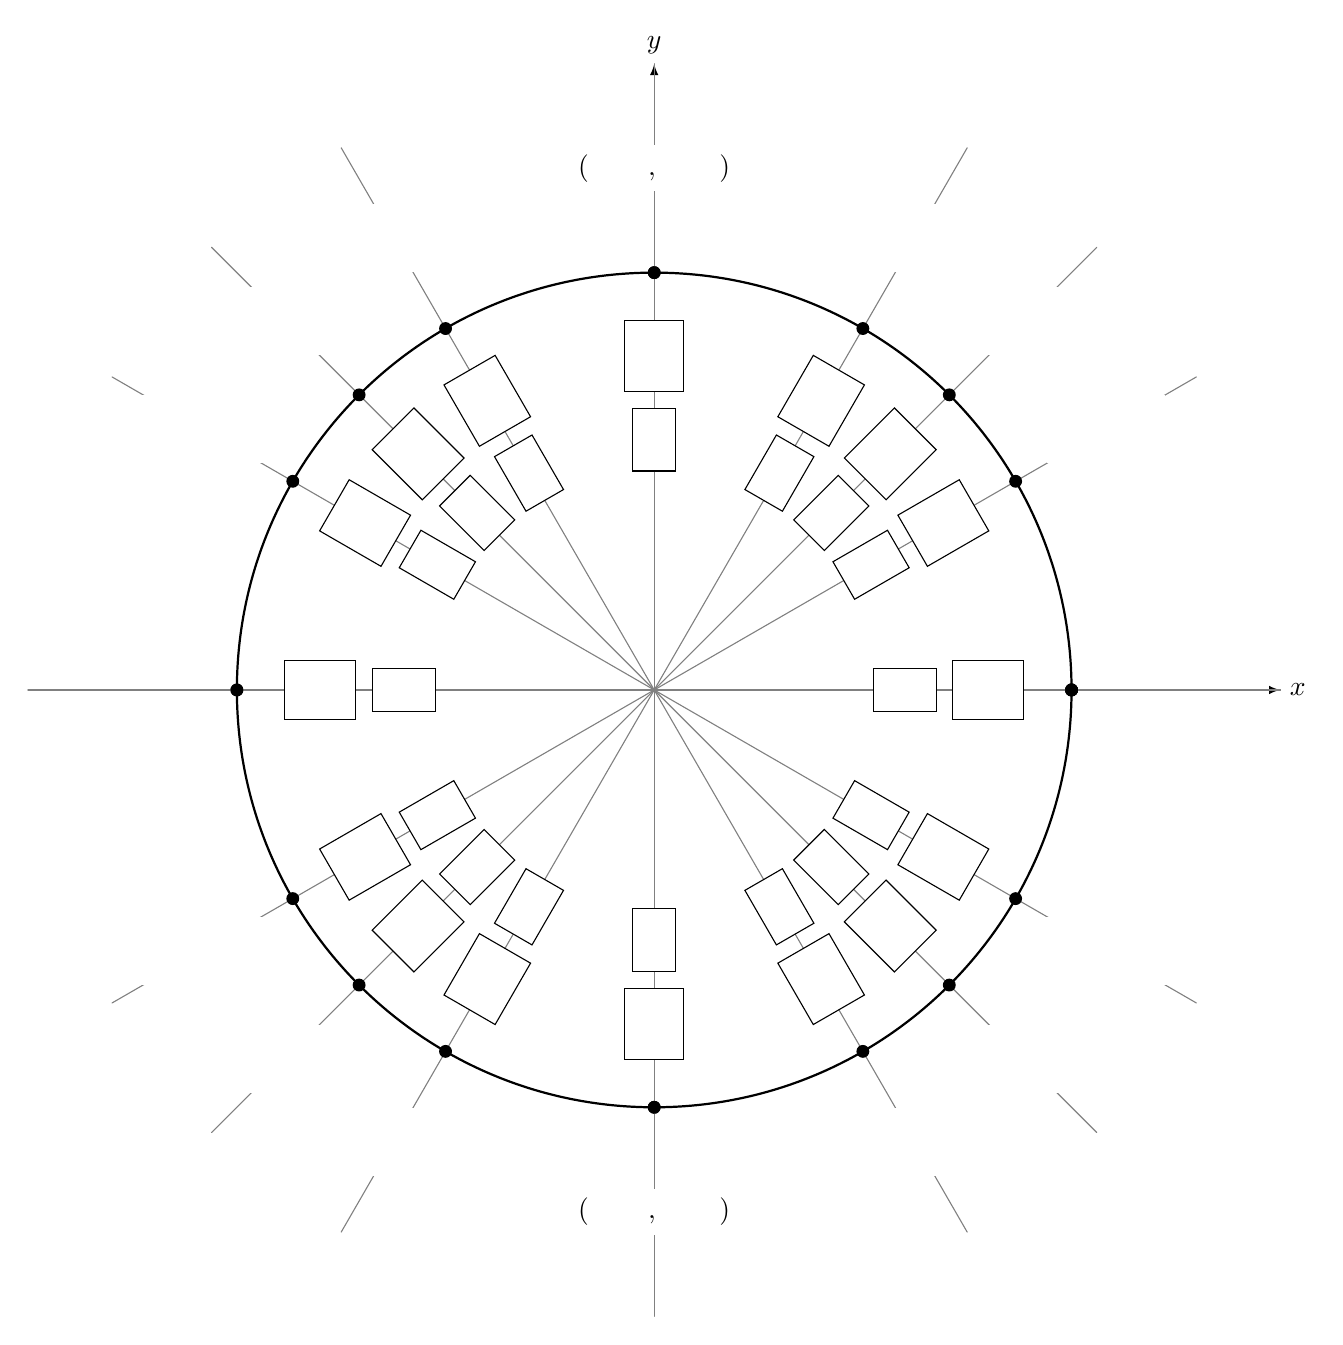
\begin{tikzpicture}[scale=5.3,cap=round,>=latex]

	% Coordinate Axes 
        \draw[->] (-1.5cm ,0cm) -- (1.5cm, 0cm) node[right, fill= white] {$x$};
        \draw[->] (0cm, -1.5cm) -- (0cm, 1.5cm) node[above, fill= white] {$y$};

	% Unit Circle
        \draw[thick] (0cm,0cm) circle(1cm);

	% '30-type' Angles
        \foreach \x in {0,30,...,360} {
                % Line from Center to Point
                \draw[gray] (0cm, 0cm) -- (\x:1.5cm);
                % Dot at Each Points
                \filldraw[black] (\x:1cm) circle(0.4pt);
                % Angles in Degrees
		\draw node[draw, fill= white, shape= rectangle, minimum height= 0.55cm, minimum width= 0.8cm, anchor= center, rotate= \x] at (\x:0.6cm) {};
		% Angle in Radians
		\draw node[draw, fill= white, shape= rectangle, minimum height= 0.75cm, minimum width= 0.9cm, anchor= center, rotate= \x] at (\x:0.8cm) {};
	}
	
	% '45-type' Angles			
	\foreach \x in {0,45,...,360} {
		% Line from Center to Point		
		\draw[gray] (0cm, 0cm) -- (\x:1.5cm);
                % Dot at Each Points			
		\filldraw[black] (\x:1cm) circle(0.4pt);
                % Angles in Degrees
		\draw node[draw, fill= white, shape= rectangle, minimum height= 0.55cm, minimum width= 0.8cm, anchor= center, rotate= \x] at (\x:0.6cm) {};
		% Angle in Radians
		\draw node[draw, fill= white, shape= rectangle, minimum height= 0.75cm, minimum width= 0.9cm, anchor= center, rotate= \x] at (\x:0.8cm) {};
	}
		
	% Horizontal/Vertical Point Placement (Better in this Format)
        \draw %(-1.25cm,0cm) node[above=1pt] {$(\hspace{.75cm},\hspace{.75cm})$}
	%(1.25cm,0cm)  node[above=1pt] {$(\hspace{.75cm},\hspace{.75cm})$}
	(0cm,-1.25cm) node[fill=white] {$(\hspace{.75cm},\hspace{.75cm})$}
	(0cm,1.25cm)  node[fill=white] {$(\hspace{.75cm},\hspace{.75cm})$};

%	% Axes Coordinates
%	\draw (-1.27cm,0cm) node[above=1pt] {$-1 \enskip\enskip\enskip 0$}
%	(1.25cm,0cm)  node[above=1pt] {$1 \enskip\enskip\enskip 0$}
%	(0.01cm,-1.25cm) node[] {$0 \quad -1$}
%	(0cm,1.25cm)  node[] {$0 \enskip\enskip\enskip 1$};
	
	% Remainder of Coordinates
	\foreach \x/\xtext/\y in {
		% Q1
		30/\frac{\sqrt{3}}{2}/\frac{1}{2},
		45/\frac{1}{\sqrt{2}}/\frac{1}{\sqrt{2}},
		60/\frac{1}{2}/\frac{\sqrt{3}}{2},
		% Q2
		150/-\frac{\sqrt{3}}{2}/\frac{1}{2},
		135/-\frac{1}{\sqrt{2}}/\frac{1}{\sqrt{2}},
		120/-\frac{1}{2}/\frac{\sqrt{3}}{2},
		% Q3
		210/-\frac{\sqrt{3}}{2}/-\frac{1}{2},
            	225/-\frac{1}{\sqrt{2}}/-\frac{1}{\sqrt{2}},
		240/-\frac{1}{2}/-\frac{\sqrt{3}}{2},
		% Q4
		330/\frac{\sqrt{3}}{2}/-\frac{1}{2},
		315/\frac{1}{\sqrt{2}}/-\frac{1}{\sqrt{2}},
		300/\frac{1}{2}/-\frac{\sqrt{3}}{2}}
		\draw (\x:1.25cm) node[color=white,fill=white] {$\left(\xtext,\y\right)$};
	
	% Label Each Angle in Radians
	\foreach \x/\xtext in {
    		30/\frac{\pi}{6},
    		45/\frac{\pi}{4},
    		60/\frac{\pi}{3},
    		90/\frac{\pi}{2},
    		120/\frac{2\pi}{3},
    		135/\frac{3\pi}{4},
    		150/\frac{5\pi}{6},
    		180/\pi,
    		210/\frac{7\pi}{6},
    		225/\frac{5\pi}{4},
    		240/\frac{4\pi}{3},
    		270/\frac{3\pi}{2},
    		300/\frac{5\pi}{3},
    		315/\frac{7\pi}{4},
    		330/\frac{11\pi}{6},
    		360/2\pi}
		\draw (\x:0.81cm) node[color=white] {$\xtext$};

	% Degree Labels (0, 30, 60, ..., 360)
	\foreach \x in {0,30,...,330} {
		\draw (\x:0.6cm) node[color=white] {\scriptsize \,$\x^\circ$};
	}
	
	% Degree Labels (0, 45, 90, ..., 360) 
	\foreach \x in {0,45,...,315} {
		\draw (\x:0.6cm) node[color=white] {\scriptsize \,$\x^\circ$};
	}	
	\end{tikzpicture}
	\]
\vfill

%\noindent {\scriptsize\itshape *Note: $\frac{1}{\sqrt{2}}= \frac{\sqrt{2}}{2}$

\end{document}